% Русская версия рукописи. Формат — «Физика твёрдого тела» (ФТТ, Ioffe):
% pdflatex + babel, аннотация без структурирования,
% литература в порядке цитирования, единицы СИ.
\documentclass[12pt,a4paper]{article}

\usepackage[T2A]{fontenc}
\ifx\pdfmapfile\undefined\else\pdfmapfile{+cm-super-t1.map}\pdfmapfile{+cm-super-t2a.map}\fi % Type 1 fonts
\usepackage[utf8]{inputenc}
\usepackage[russian]{babel}
\usepackage{amsmath,amssymb}
\usepackage{graphicx}
% имена файлов в разделе о доступности данных переносятся по подчёркиваниям
\usepackage{url}
\usepackage{placeins}
\usepackage[left=2.5cm,right=2cm,top=2.5cm,bottom=2.5cm]{geometry}
\usepackage{indentfirst}
\setlength{\parindent}{1.25cm}
\linespread{1.15}
% Дополнительный проход абзацев, которые иначе не укладываются в строку
% (длинные неразрывные формулы и латинские названия).
\setlength{\emergencystretch}{1em}

\begin{document}

\begin{center}
{\large\bfseries Атомистические оценки магнитострикционного механизма\\
магнитной памяти пластичности в сплавах Al--Mg--Si\\
с железосодержащими включениями}

\medskip
{И.\,Е.\,Михайловский, Д.\,Е.\,Пшонкин}

\smallskip
{\itshape Московский политехнический университет, Москва, Россия}
\end{center}

\medskip

\noindent\textbf{Аннотация.}
Методом молекулярной динамики исследуется, как предварительная выдержка
сплава Al--Mg--Si с включениями Al$_{13}$Fe$_4$ в постоянном магнитном поле
влияет на пластическую деформацию при одноосной ползучести. Включение
удлинено вдоль поля на 0{,}194\% --- деформация, отвечающая оценённому в
ранних экспериментах межфазному напряжению 147~МПа, --- и удерживается при
этой деформации, пока матрица релаксирует. Разрешённое касательное
напряжение в матрице достигает 15~МПа непосредственно над включением и в
пределах 80~\AA{} спадает до разрешающей способности расчёта. При сдвиговом
нагружении существующая пара дислокаций разрывается начиная с 95--105~МПа, а
новых дислокаций на границе в недеформированной ячейке не образуется вплоть
до 400~МПа. Двухмасштабная оценка воспроизводит наблюдаемый прирост
ползучести 25\% при рассчитанных напряжениях для активационных объёмов,
измеренных для Al--Mg--Si, --- при условии, что включения действительно
деформируются на 0{,}194\%; измеренная магнитострикция сплавов Fe--Al в
двадцать раз меньше, а сохранение эффекта после снятия поля упругим
напряжением не объясняется.

\noindent\textbf{Ключевые слова:} магнитопластичность, магнитная память,
ползучесть, молекулярная динамика, сплавы Al--Mg--Si, Al$_{13}$Fe$_4$,
межфазные напряжения, дислокации, закрепление дислокаций примесями.

\section{Введение}

Слабые магнитные поля, энергия которых в расчёте на атом ничтожна по
сравнению с тепловой энергией $kT$, тем не менее изменяют пластичность
немагнитных кристаллов; совокупность таких наблюдений известна как
магнитопластический эффект [1,\,2]. Алюминиевые сплавы с железосодержащими
включениями занимают в этом ряду особое место: если такое включение
ферромагнитно, они допускают на первый взгляд простой механический путь от
поля к пластическому течению --- поле намагничивает включение,
магнитострикция (изменение формы намагниченного тела) деформирует его, и
напряжение, вызванное несоответствием между деформированным включением и
окружающей матрицей, передаётся матрице. Вопрос о том, действительно ли
включения в этих сплавах ферромагнитны, рассматривается в разделе~5.1. Серия экспериментов на промышленном сплаве Al--Mg--Si с
железосодержащими микровключениями подробно описала явление: 30-минутная
выдержка в поле $B = 0{,}4$--$0{,}7$~Тл, проводимая \emph{до} механических
испытаний, увеличивает последующую деформацию ползучести (медленного
деформирования под постоянной нагрузкой) при 160~МПа и комнатной температуре
примерно на четверть, в несколько раз повышает тепловыделение при
деформировании и смещает коэффициент Тейлора--Куинни --- долю работы
пластической деформации, выделяющуюся в виде тепла, --- с 0{,}07 до 0{,}25
[3--6]. Поскольку эффект сохраняется после снятия поля, его называют
«магнитной памятью» пластичности [4].

Предложенная в этих работах интерпретация опирается на единственную оценку.
Напряжение на границе включения с матрицей, создаваемое магнитострикцией
включения и полученное из величины поля через эмпирический коэффициент
пропорциональности, оценено примерно в 147~МПа при $B = 0{,}7$~Тл [5]. Это
превышает предел текучести матрицы 120~МПа, откуда и сделан вывод, что
матрица вокруг каждого включения пластически деформируется, а плотность
дислокаций --- линейных дефектов кристаллической решётки, движение которых и
составляет пластическое течение, --- возрастает. Эта цепочка рассуждений
никогда не проверялась на том масштабе, на котором она должна действовать.
Возникает ли в матрице напряжение такой величины, на каком расстоянии от
границы оно сохраняется и способно ли оно зарождать дислокации или приводить
в движение уже имеющиеся --- всё это вопросы об ангстремах и пикосекундах,
то есть о естественной области классической молекулярной динамики (МД), в
которой атомы движутся по уравнениям Ньютона под действием сил, задаваемых
межатомным потенциалом.

В настоящей работе магнитострикционный механизм подвергнут количественной
атомистической проверке на границе между алюминием и интерметаллидом
Al$_{13}$Fe$_4$. Магнитное поле в классической МД непосредственно не
представлено, поэтому его действие задаётся механически: по данным более
ранней экспериментальной работы [5] включение считается удлинённым вдоль
направления поля на $\varepsilon = 1{,}94\cdot10^{-3}$ (0{,}194\%) при
неизменном объёме --- это деформация, отвечающая оценённому там напряжению
на границе 147~МПа. Прямое воспроизведение макроскопического эффекта в
расчётной ячейке не предпринимается; причина изложена в разделе
«Обсуждение». Вместо этого каждое звено предполагаемой цепочки исследуется в
отдельности. Рассчитываются: поле напряжений, которое удлинённое включение
создаёт в матрице, и его затухание с расстоянием от границы; приложенное
сдвиговое напряжение, при котором уже имеющаяся в матрице дислокация
приходит в движение, и образуются ли на границе новые дислокации вплоть до наибольшего приложенного напряжения; сопротивление, которое растворённые в алюминии атомы Mg и Si
оказывают движению дислокации. Затем цепочка замыкается с противоположного
конца: двухмасштабная оценка даёт напряжение на границе, которое
\emph{требуется} для измеренного прироста ползучести на 25\% при термически
активированном скольжении --- движении дислокаций, при котором препятствия
преодолеваются с помощью тепловых флуктуаций, так что скорость скольжения
экспоненциально зависит от напряжения, --- и при затухании упругого поля
вне деформированного включения как $r^{-3}$ [7].

\section{Методика расчёта}

\subsection{Расчётная ячейка границы}

Все расчёты выполнены в пакете LAMMPS (версия 22.07.2025, сборка
KOKKOS\slash CUDA для графических процессоров) [8]. Межатомные силы заданы
потенциалом 2NN-MEAM (модифицированный метод погружённого атома с учётом
вторых соседей) Елинека и др. для системы Al--Si--Mg--Cu--Fe [9] --- единым
потенциалом, который описывает все атомы ячейки, в том числе атомы по обе
стороны границы, одним набором правил взаимодействия.

Матрица --- ГЦК (гранецентрированный кубический) алюминий
($a = 4{,}05$~\AA{}). Её ориентация, $x\parallel[1\bar{1}0]$,
$y\parallel[11\bar{2}]$, $z\parallel[111]$, продиктована системой скольжения
ГЦК-алюминия: дислокации в алюминии движутся по плоскостям $\{111\}$ вдоль
направлений $\langle110\rangle$, и при таком выборе плоскость скольжения
(111) параллельна границе, а направление скольжения $[1\bar{1}0]$ лежит
вдоль $x$. Краевая дислокация (край лишней атомной полуплоскости, вставленной
в кристалл) с вектором Бюргерса $\tfrac{1}{2}[1\bar{1}0]$ --- трансляцией
решётки, задающей переносимое ею смещение, $|\mathbf{b}| = 2{,}86$~\AA{}, ---
и линией вдоль $y$ при этом проходит через всю ширину ячейки, представляя
бесконечно длинную прямолинейную дислокацию, и скользит вдоль $x$
параллельно границе; именно такое движение и должен вызывать проверяемый
механизм.

Включение --- моноклинный интерметаллид Al$_{13}$Fe$_4$ со структурой из
работы [10]. Оно построено как плоский слой толщиной 20~\AA{}, несущий на
верхней поверхности полуэллиптический выступ (далее --- гребень) с полуосями
35~\AA{} вдоль $x$ и 20~\AA{} вдоль $z$, протянутый через всю ячейку вдоль
$y$. Гребень необходим: плоский деформированный слой, занимающий всю ячейку,
снимает нормальное напряжение простым расширением вверх, и именно
искривлённые края гребня создают в матрице неоднородное поле напряжений ---
так же, как его создавала бы кривизна поверхности реальной частицы. Плоский слой оставлен недеформированным, деформацию несёт только гребень
(раздел~2.2).

Вдоль $x$ и $y$ ячейка периодична: атом, выходящий через одну грань, входит
через противоположную, так что ячейка представляет неограниченную в плоскости
границу. Размеры в плоскости ($L_x = 154{,}64$~\AA{}, $L_y = 64{,}48$~\AA{}: 54 и
13 периодов решётки алюминия, десять и восемь ячеек Al$_{13}$Fe$_4$) выбраны
так, чтобы обе решётки были периодичны в плоскости. Малое остаточное
несоответствие ($-0{,}22\%$ вдоль $x$, $-0{,}26\%$ вдоль $y$) отнесено к
включению и одинаково в деформированной и контрольной ячейках, поэтому при их
сравнении оно сокращается в первом приближении. Атомы алюминия, оказавшиеся ближе
2{,}2~\AA{} к атому включения (с учётом периодических образов), удалены;
наименьшее межатомное расстояние в полученной структуре составляет
2{,}22~\AA{}. Толщина слоя алюминия над плоскостью границы 129~\AA{} (56 атомных
плоскостей (111)), ячейка в целом содержит 91\,428 атомов (72\,532 в матрице
и 18\,896 во включении); вдоль $z$ она ограничена сверху свободной
поверхностью и 17~\AA{} вакуума, снизу --- слоем толщиной 6~\AA{}, атомы
которого закреплены (рис.~\ref{fig:cell}).

Включение сцеплено с матрицей. Атомы по обе стороны границы взаимодействуют
через один и тот же потенциал, никаких ограничений или искусственной связи на
границе не вводится, и граница не проскальзывает и не раскрывается иначе, чем
через смещения атомов, допускаемые самим потенциалом. Контрольная структура релаксируется в три стадии: минимизация энергии
методом сопряжённых градиентов (атомы переводятся в положения минимума
энергии без теплового движения), 6~пс молекулярной динамики при 300~К с
последующим охлаждением до 0{,}5~К за 12~пс, снимающие длинноволновые моды
слоя, недоступные одной минимизации, и заключительная минимизация до силы
0{,}05~эВ/\AA{} (2-норма по всем атомам). Деформированная ячейка строится из
этого релаксированного состояния (раздел~2.2) и минимизируется до
0{,}02~эВ/\AA{}.

\begin{figure}[!htbp]
\centering
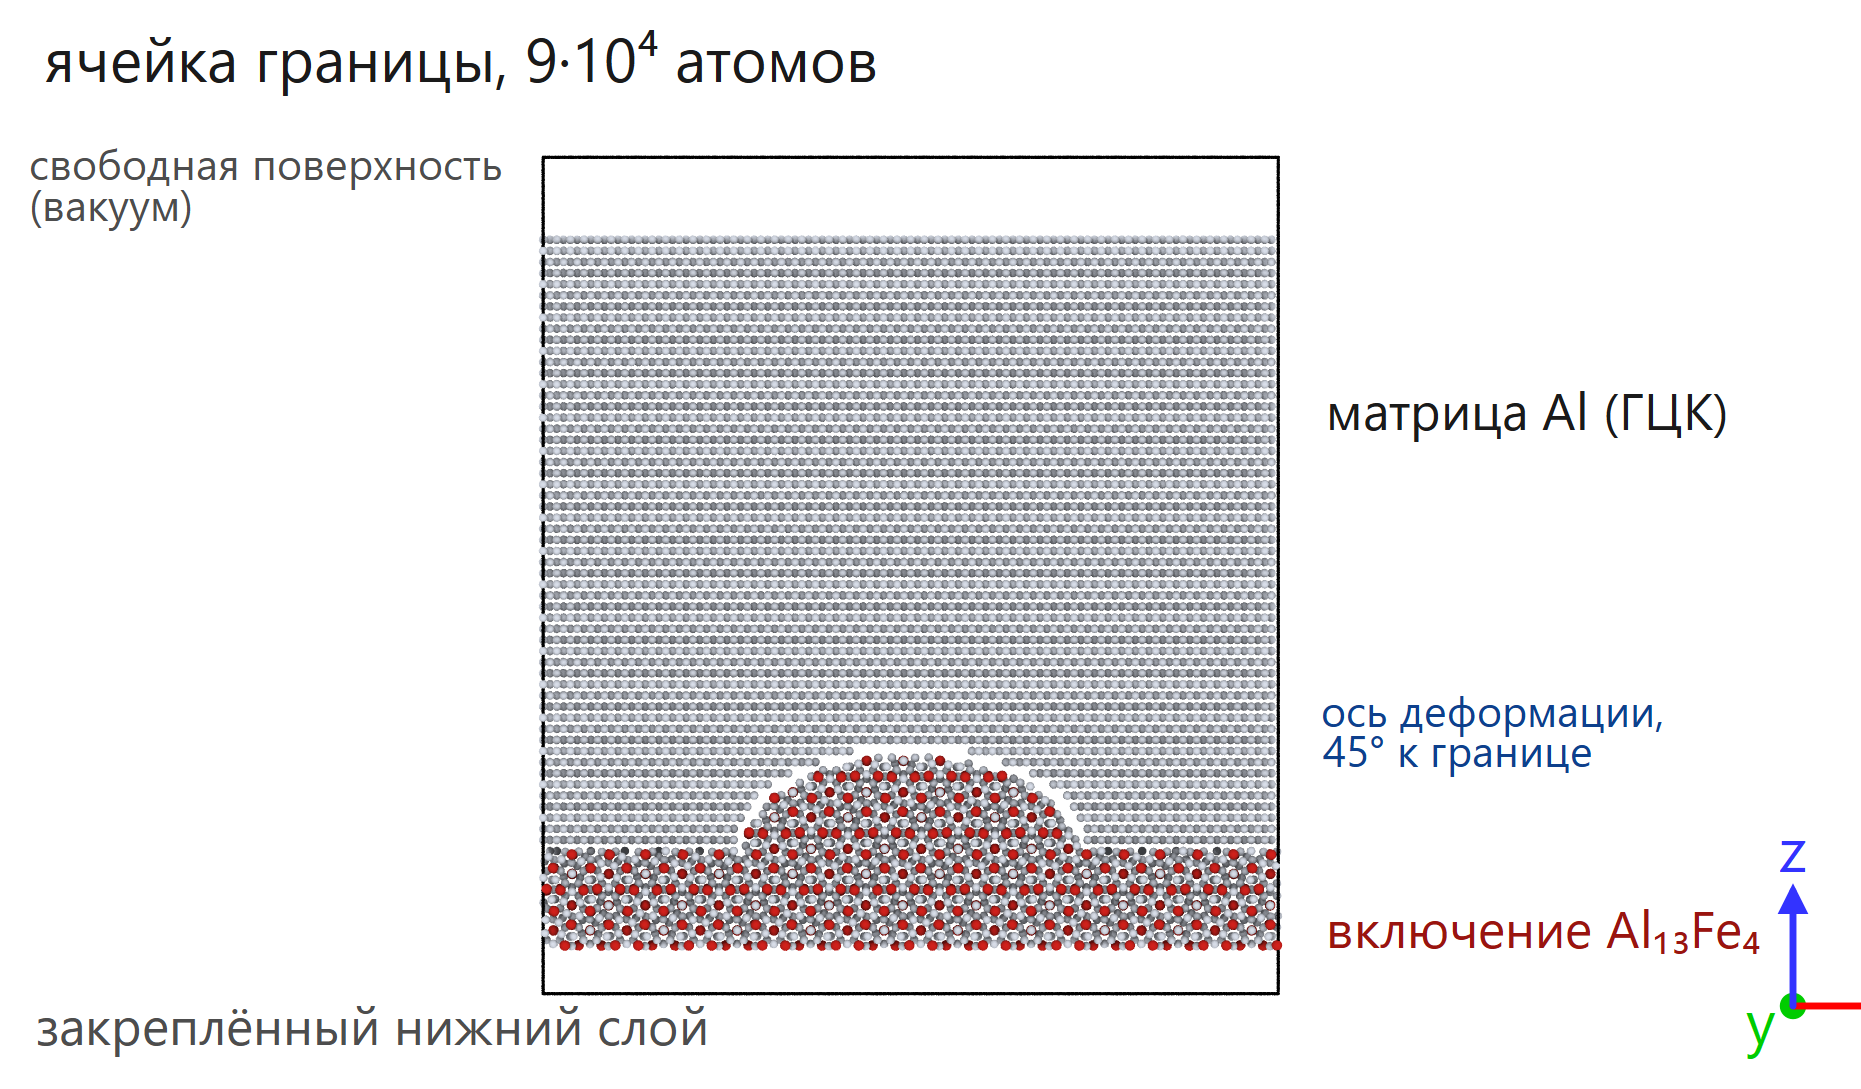
\includegraphics[width=0.92\linewidth]{fig_cell_interface_ru}
\caption{Расчётная ячейка границы в проекции вдоль $y$ (плоскость
$x$--$z$). Серым показана матрица алюминия --- 129~\AA{} ГЦК-алюминия с
осями $x = [1\bar{1}0]$, $y = [11\bar{2}]$, $z = [111]$, так что граница
параллельна плоскости скольжения (111), а $x$ --- направление скольжения.
Красным --- включение Al$_{13}$Fe$_4$: плоский слой с полуэллиптическим
гребнем шириной 70~\AA{} и высотой 20~\AA{}. Нижние 6~\AA{} включения
закреплены; над алюминием --- вакуум. Ячейка периодична вдоль $x$ и $y$.
Наложенное удлинение включения направлено под $45^{\circ}$ к границе в
плоскости $x$--$z$.}
\label{fig:cell}
\end{figure}

\subsection{Представление действия поля}

Молекулярная динамика --- классическая механика, и само магнитное поле в
расчёте отсутствует. Его действие представлено механически --- деформацией,
которую оно, по предположению, вызывает во включении. Вслед за
предшествующими экспериментальными работами [3--6], в которых поле действует
через магнитострикцию, то есть удлинение включения вдоль направления поля,
включение принято удлиняющимся вдоль направления поля $\mathbf{u}$ на
$\varepsilon = 1{,}94\cdot10^{-3}$ (0{,}194\%) --- упругую деформацию
$\sigma_m/E_{\mathrm{Al}}$ (при $E_{\mathrm{Al}} = 75{,}7$~ГПа), отвечающую оценённому в этих работах напряжению
на границе $\sigma_m = 147$~МПа [5], --- при постоянном объёме: удлинение
$\varepsilon$ вдоль $\mathbf{u}$ и сжатие на $\varepsilon/2$ вдоль двух
перпендикулярных направлений. В тензорной записи
\begin{equation}
\varepsilon^{*}_{ij}
  = \tfrac{3}{2}\,\varepsilon\!\left(u_i u_j - \tfrac{1}{3}\delta_{ij}\right),
\qquad \operatorname{tr}\varepsilon^{*} = 0,
\end{equation}
где $\delta_{ij}$ равно 1 при $i = j$ и 0 в остальных случаях, а нулевой след
выражает постоянство объёма. В теории упругости включений деформацию такого
рода --- ту, которую включение приняло бы, будучи свободным от матрицы, ---
называют собственной деформацией [7]; ниже этот термин употребляется именно в
этом смысле. Принятое значение существенно превышает магнитострикцию,
измеренную в сплавах Fe--Al [11,\,12]; оно используется потому, что это та
амплитуда, которую предполагает сам предложенный механизм, и механизм
проверяется при ней.

Направление $\mathbf{u}$ наклонено под углом $45^{\circ}$ к нормали границы
в плоскости $x$--$z$. Причина геометрическая. При $\mathbf{u}$ вдоль нормали
$z$ наложенная деформация не создаёт на системе скольжения $(111)[1\bar{1}0]$
никакого касательного напряжения: фактор Шмида (геометрический множитель,
переводящий напряжение в касательное напряжение на данной системе скольжения)
равен нулю точно, и на дислокацию, скользящую параллельно границе, не
действовала бы никакая сила. При $45^{\circ}$ сдвиговая составляющая
наложенной деформации на плоскости скольжения максимальна,
$\varepsilon^{*}_{xz} = \tfrac{3}{4}\varepsilon = 1{,}46\cdot10^{-3}$. В
поликристалле на поле откликаются те зёрна, чьи плоскости скольжения
благоприятно наклонены к нему, и наклонённая ячейка представляет именно эту
часть зёрен. Наклон одинаков во всех ячейках.

Деформация задаётся смещением каждого атома гребня относительно центра
гребня пропорционально его положению,
$\mathbf{r} \rightarrow \mathbf{r} + \varepsilon^{*}\!\cdot\!\mathbf{r}$, что
однородно растягивает гребень вдоль $\mathbf{u}$ и сжимает поперёк
$\mathbf{u}$. Плоский слой под гребнем оставлен недеформированным. Он
проходит через всю периодическую ячейку, а слой, периодичный в своей
плоскости, нельзя когерентно сдвинуть: удерживаемый при сдвиге формулы~(1),
он имел бы поверхность в виде пилы со ступенькой
$\varepsilon^{*}_{xz}L_x = 0{,}22$~\AA{} на границе ячейки, и весь слой
алюминия над ним оказался бы растянут вдоль $z$ примерно на
$\varepsilon^{*}_{xz}$ --- напряжение порядка 150~МПа по всей ячейке, что и
наблюдалось при такой попытке. Гребень --- та частица, поле которой
измеряется; слой лишь замыкает ячейку. Межатомный потенциал не изменяется. Поле напряжений,
создаваемое деформированным включением, получается как разность между ячейкой
с деформированным включением и контрольной ячейкой без деформации,
минимизированными из одинаковых исходных структур в одинаковых условиях.
Рассчитаны два варианта, различающиеся тем, позволено ли включению
релаксировать.

В варианте \emph{с удерживаемой деформацией} каждый атом включения ---
гребень в смещённом положении, плоский слой в исходном --- удерживается
жёсткой пружиной (жёсткость 20~эВ/\AA$^{2}$, что удерживает атом в пределах
примерно 0{,}01~\AA{} от этого положения), пока матрица релаксирует вокруг
него, так что гребень сохраняет деформацию~(1) на всём протяжении расчёта. В
соответствующей контрольной ячейке пружины подключены точно так же, поэтому
в разности двух ячеек они сокращаются. Эта ячейка даёт поле напряжений
частицы, поддерживающей свою собственную деформацию. Под действием сил, возникающих на границе, атомы включения отходят от
заданных положений примерно на 0{,}01~\AA{}, и гребень сохраняет
$0{,}97\pm0{,}004$ наложенной деформации (измерено так же, как описано ниже для
свободного варианта).

В \emph{свободном} варианте пружин нет, и включение вольно снять наложенную
деформацию. Оно снимает её в значительной мере: после минимизации гребень,
который и создаёт измеряемое в матрице поле, сохраняет 0{,}2--0{,}4
наложенной деформации ($0{,}20 \pm 0{,}11$ и $0{,}44 \pm 0{,}10$ в двух
минимизациях, обе остановлены до полной сходимости). Доля измеряется как проекция остаточного искажения
Fe-подрешётки включения на $\varepsilon^{*}$, найденного подгонкой смещений
между деформированной и контрольной ячейками методом наименьших квадратов;
погрешность --- стандартная ошибка этой подгонки. Свободный вариант
показывает, что делает включение, когда его деформацию ничто не удерживает;
его поле напряжений --- релаксированный отклик, а не поле включения,
поддерживающего деформацию, и с порогами движения дислокаций ниже
сопоставляется удерживаемый вариант.

\emph{Контрольная} ячейка деформации не содержит. Это сама релаксированная
структура раздела~2.1; деформированная ячейка строится из неё,
минимизируется с тем же допуском и сравнивается с ней атом за атомом, так
что остаточное несоответствие решёток раздела~2.1, состояние прослойки на
границе и длинноволновая деформация слоя общие для обеих и в разности
сокращаются. Ячейки границы дают профиль напряжений в матрице и длину его
затухания. Напряжения, при которых дислокации приходят в движение, получены
отдельно, в нагружаемых ячейках раздела~2.3, и служат лишь порогами, с
которыми сопоставляется этот профиль.

\subsection{Нагружаемые ячейки и схема нагружения}

Напряжения, при которых движутся дислокации, измерены в двух ячейках,
нагружаемых сдвигом в динамике при 300~К.

Первая --- ячейка границы раздела~2.1 с заранее введённой парой краевых
дислокаций, помещённой рядом с гребнем включения; всего 91\,428 атомов (рис.~\ref{fig:loading}). Пара представляет собой
дислокационный диполь: две параллельные дислокации противоположного знака,
поля напряжений которых притягиваются, так что в однородном ненагруженном кристалле пара устойчива и остаётся там, где помещена, пока приложенное напряжение не превысит уровень, при котором
партнёры могут пройти друг мимо друга. Обе дислокации лежат вдоль $y$ и
скользят по плоскостям (111), параллельным границе. Партнёры смещены друг относительно друга на 23{,}4~\AA{} вдоль $x$ и на
десять межплоскостных расстояний (111), 23{,}4~\AA{}, вдоль $z$, так что
соединяющая их линия наклонена к плоскостям скольжения под $45^{\circ}$. Две
краевые дислокации противоположного знака в плоскостях скольжения на
расстоянии $h$ притягиваются с касательным напряжением до
$\mu b/[8\pi(1-\nu)h]$, что при $h = 23{,}4$~\AA{} составляет 198~МПа (при
$\mu = 26{,}5$~ГПа, $\nu = 0{,}347$, $b = 2{,}864$~\AA{}); это приложенное
напряжение, при котором они прошли бы друг мимо друга в неограниченном
кристалле. Нижний партнёр помещён в 27~\AA{} за подножием гребня и в
29~\AA{} над плоскостью границы, верхний --- на 23~\AA{} выше и на 23~\AA{}
ближе к гребню. Ячейка нагружается касательным напряжением, линейно растущим от 0
до 400~МПа за 96~пс после 5~пс выдержки при нулевом напряжении. Напряжение
прикладывается как однородная сила вдоль $x$ к атомам верхних атомных слоёв,
реакцию воспринимает закреплённый нижний слой; скорость роста включается
плавно в течение первых 16~пс, чтобы не возбудить низшее сдвиговое колебание
слоя. Нагружение значительно быстрее любого лабораторного испытания
(эффективная скорость деформации порядка $10^{8}$~с$^{-1}$), поэтому
полученные пороги --- верхние оценки относительно медленного нагружения.
Выполнены три рампы: недеформированная ячейка со свободно релаксирующим
включением --- до 400~МПа за 96~пс; недеформированная и деформированная
ячейки с включением, удерживаемым пружинами раздела~2.2, --- при той же
скорости роста до 145~МПа за 40~пс (эта пара и сравнивает деформированный
гребень с недеформированным).

Вторая ячейка включения не содержит. Это слой матрицы сплава той же
ориентации, 92\,800 атомов (91\,315~Al, 928~Mg, 557~Si;
$114{,}6\times49{,}6\times291$~\AA{}), в котором 1{,}0~ат.\%~Mg и 0{,}6~ат.\%~Si размещены случайно по узлам решётки
и который содержит один краевой диполь с партнёрами на параллельных
плоскостях скольжения на расстоянии 206~\AA{}; их взаимное притяжение
отвечает касательному напряжению $\mu b/[8\pi(1-\nu)h] \approx 22$~МПа,
малому по сравнению с прикладываемыми напряжениями. Перед нагружением
структура минимизируется по энергии и выводится на 300~К. Эта ячейка
нагружается ступенями: постоянные касательные напряжения 45, 55, 65 и
75~МПа, каждое удерживается 30~пс и включается плавно за 4~пс, после 10~пс
при нулевом напряжении. Ступени вместо линейного роста выбраны потому, что
дислокация, удерживаемая атомами примеси, движется, отрываясь от них, --- это
термически активируемое событие, время ожидания которого зависит от
напряжения; выдержка при постоянном напряжении в течение заданного времени
проверяет, отрывается ли дислокация при данном уровне, и напряжение
поднимается ступенями, чтобы найти уровень, при котором это происходит.
Ячейка чистого алюминия той же геометрии служит эталоном без примесей.

В обеих ячейках уравнения движения интегрируются с шагом по времени 1~фс ---
около сотой доли периода колебаний атома. Температура поддерживается на
уровне 300~К термостатом Нозе--Хувера (время релаксации 0{,}1~пс), который
удерживает среднюю кинетическую энергию незакреплённых атомов на заданном
значении слабой обратной связью по их скоростям. Дислокации вводятся
построением Вольтерры: кристалл разрезается по полуплоскости, две стороны
разреза смещаются друг относительно друга на один вектор Бюргерса и вновь
соединяются, причём поле смещений согласуется с периодичностью ячейки.
Дислокационное содержимое каждой исходной структуры проверяется алгоритмом
выделения дислокаций (DXA) [13], который находит дислокационные линии в
атомной конфигурации и определяет их векторы Бюргерса, в реализации пакета
OVITO [14].

\begin{figure}[!htbp]
\centering
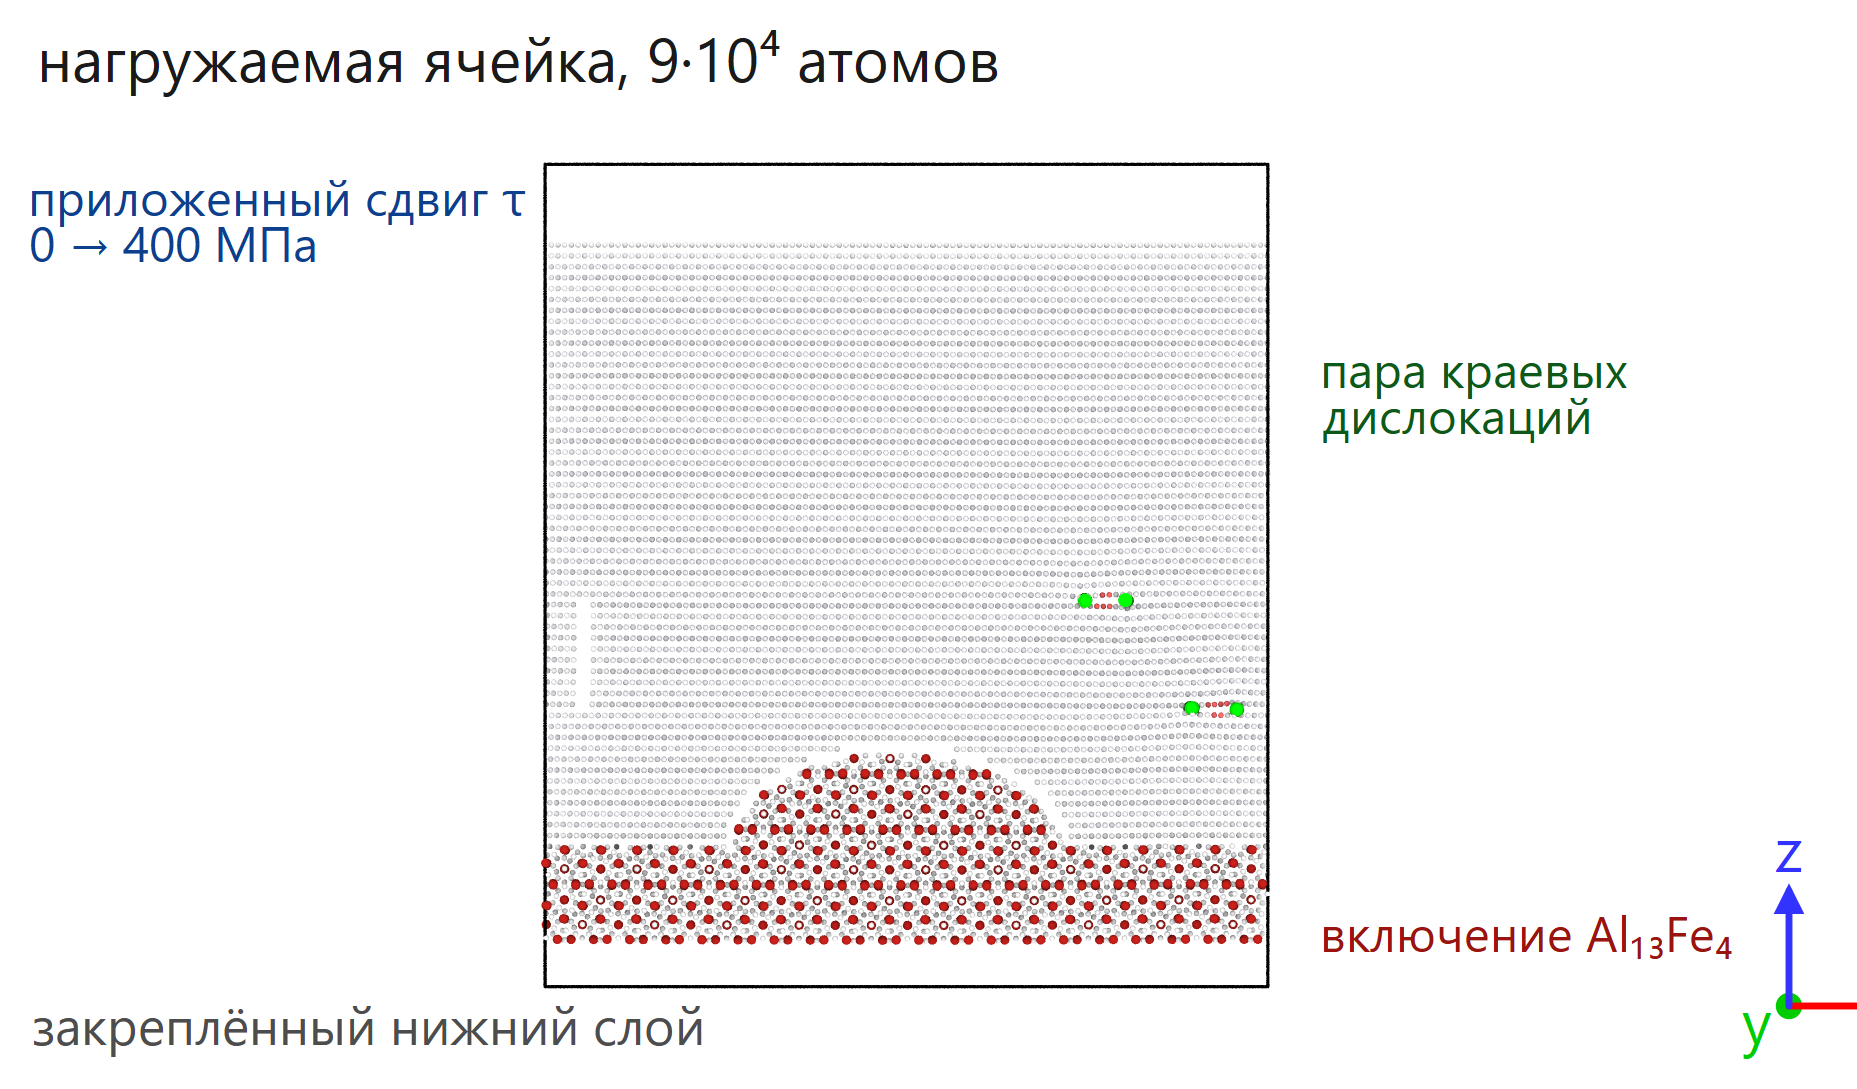
\includegraphics[width=0.92\linewidth]{fig_cell_loading_ru}\\[2mm]
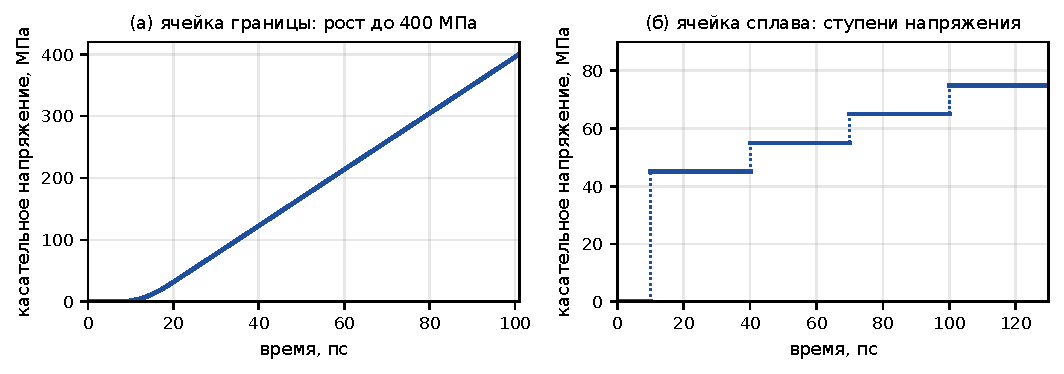
\includegraphics[width=0.92\linewidth]{fig_loading_programme_ru}
\caption{Нагружаемая ячейка границы (вверху) и две программы нагружения
(внизу). Вверху: ячейка рис.~\ref{fig:cell} с парой краевых дислокаций
противоположного знака рядом с гребнем (зелёным показаны линии дислокаций,
найденные дислокационным анализом; атомы совершенной решётки приглушены), обе
в плоскостях скольжения (111), параллельных границе. Касательное напряжение
$\tau$ вдоль $x$ прикладывается однородной силой к верхним атомным слоям и
воспринимается закреплённым нижним слоем. Внизу: программы напряжения --- для
этой ячейки линейный рост от 0 до 400~МПа за 96~пс после 5~пс при нулевом напряжении (удерживаемые ячейки нагружались с той же скоростью до 145~МПа) (а); для ячейки сплава без включения (раздел~3.3) ступени 45, 55,
65 и 75~МПа по 30~пс каждая после 10~пс без нагрузки (б).}
\label{fig:loading}
\end{figure}

\subsection{Вычисление напряжений}

Локальные напряжения получены из поатомного вириального напряжения ---
атомного аналога механического напряжения, вычисляемого для каждого атома из
сил между ним и его соседями и делённого на атомный объём
$\Omega = 16{,}61$~\AA{}$^3$: $\sigma_{ij} = -\langle W_{ij}\rangle/\Omega$.
Напряжение отдельного атома испытывает тепловые флуктуации в несколько ГПа,
поэтому никакая скалярная мера не образуется поатомно. Сначала шесть
компонент тензора усредняются по слою толщиной 4~\AA{}, параллельному границе
(а в динамических расчётах --- и по кадрам), и лишь затем из усреднённого
тензора образуются две скалярные меры: напряжение фон Мизеса --- единственное положительное число,
характеризующее сдвиговую часть напряжённого состояния и входящее в критерий
текучести пластичного металла, --- и разрешённое
касательное напряжение --- касательное напряжение, действующее на данной
плоскости скольжения в данном направлении скольжения. Через
$\mathrm{RSS}_{\max}$ обозначено наибольшее разрешённое касательное
напряжение среди двенадцати систем скольжения $\{111\}\langle110\rangle$
матрицы, то есть касательное напряжение на наиболее благоприятно
ориентированной системе.

Профили напряжений $\sigma(r)$ строятся как функции расстояния $r$ от
плоскости границы по слоям толщиной 4~\AA{} только по атомам матрицы,
лежащим выше вершины гребня, так что $r$ измеряет расстояние от поверхности
включения. Поле деформированного включения есть разность между
деформированной и контрольной ячейками, слой за слоем. В структурах после
минимизации энергии теплового движения нет, и уровень шума этой разности
задаётся остаточным разбросом от слоя к слою вдали от границы: по области
$r \geq 60$~\AA{} среднее $\Delta\mathrm{RSS}_{\max}$ составляет
$2{,}5 \pm 0{,}5$~МПа (среднее и стандартное отклонение по тринадцати
слоям) --- разрешающая способность расчёта, ниже которой поле не
разрешается.

\section{Результаты}

\subsection{Поле напряжений у границы и его затухание}

На рис.~\ref{fig:sigma} показано, как напряжение в матрице алюминия меняется
с расстоянием $r$ от плоскости границы в двух ячейках границы
(раздел~2.1): в контрольной, где гребень не деформирован, и в ячейке, где
гребень удлинён вдоль направления поля на $\varepsilon = 1{,}94\cdot10^{-3}$
и удерживается в этом состоянии (раздел~2.2). Деформированная ячейка
построена из релаксированной контрольной смещением атомов гребня и затем
минимизирована, так что две ячейки различаются только деформацией гребня.
Матрица разбита на слои толщиной 4~\AA{}, параллельные границе; шесть
компонент тензора напряжений усреднены по атомам алюминия каждого слоя, и
лишь из усреднённого тензора образованы инварианты (раздел~2.4).
Используются два усреднения. Первое охватывает всю ячейку по $x$ и $y$, то
есть область как над гребнем, так и рядом с ним; второе ограничено окном
шириной 20~\AA{} вокруг оси гребня --- это напряжение, которое матрица
испытывает непосредственно над включением. Гребень --- полуэллиптический
выступ включения с полуосями 35~\AA{} вдоль $x$ и 20~\AA{} вдоль $z$
(рис.~\ref{fig:cell}) --- имеет вершину при $r = 20$~\AA{}, так что над
вершиной расстояние до ближайшей поверхности включения равно
$d = r - 20$~\AA{}.

\begin{figure}[!htbp]
\centering
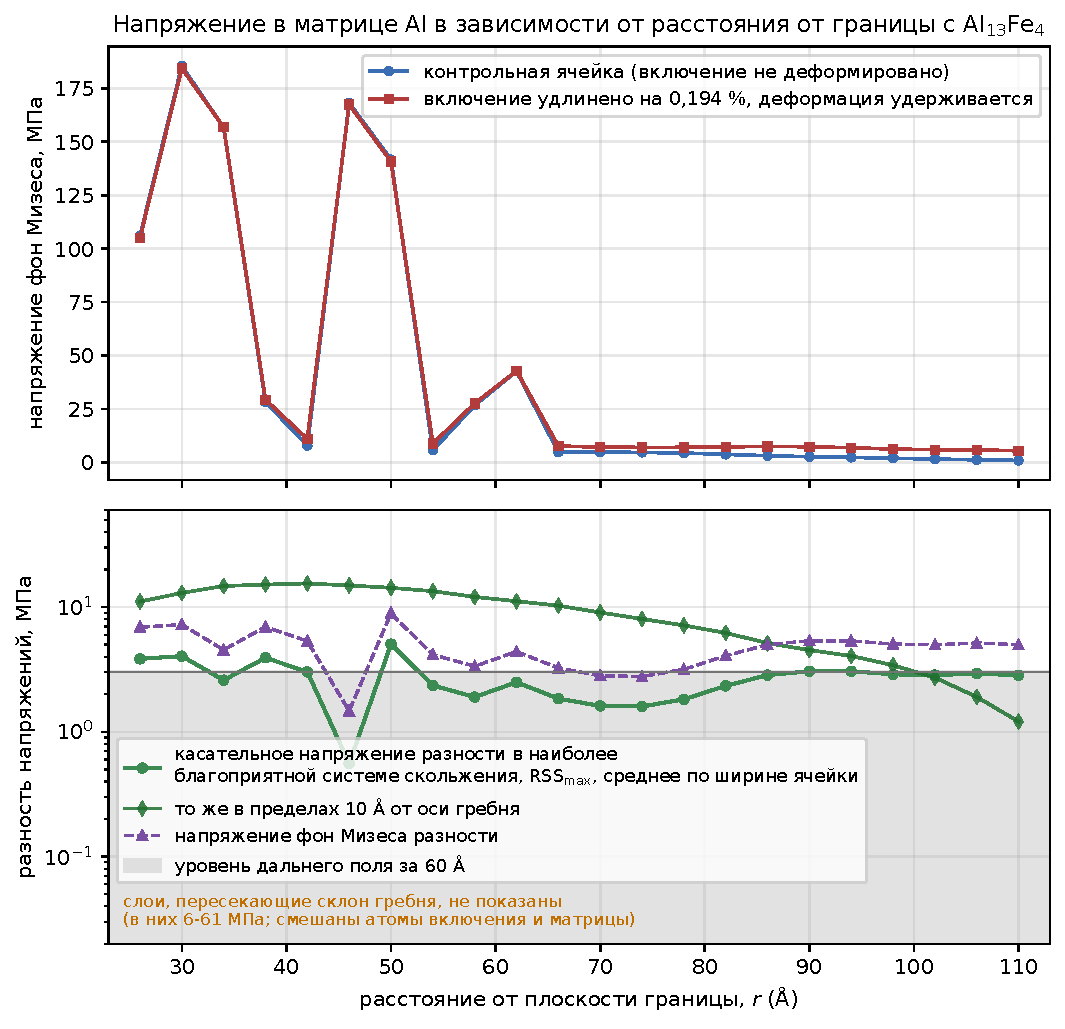
\includegraphics[width=0.80\linewidth]{fig_sigma_profile_ru}
\caption{Напряжение в матрице алюминия в зависимости от расстояния $r$ от
плоскости границы в двух ячейках границы (91\,428 атомов): в контрольной
ячейке с недеформированным гребнем и в ячейке, где гребень удлинён вдоль
направления поля на 0{,}194\% и удерживается при этой деформации. Матрица
разбита на слои толщиной 4~\AA{}, параллельные границе; шесть компонент
тензора напряжений усредняются по атомам алюминия каждого слоя, и лишь
затем из усреднённого тензора образуются инварианты. Сверху: напряжение фон
Мизеса в каждой из ячеек; 100--190~МПа непосредственно над вершиной гребня,
присутствующие в обеих ячейках, --- это напряжение когерентности сцеплённой
границы между двумя кристаллами с разными межатомными расстояниями; кривые
совпадают. Снизу: разность $\Delta\sigma_{ij} = \sigma_{ij}(\varepsilon) -
\sigma_{ij}(0)$ как касательное напряжение, спроецированное на наиболее
благоприятную из двенадцати систем скольжения ГЦК-алюминия,
$\mathrm{RSS}_{\max}$, в среднем по всей ширине ячейки (кружки) и в
пределах 10~\AA{} от оси гребня (ромбы), а также напряжение фон Мизеса
разностного тензора. Затенённая область отмечает напряжения ниже 3~МПа: уровень среднего по
ширине за 60~\AA{} с его разбросом, $2{,}5 \pm 0{,}5$~МПа, разрешающая
способность расчёта для длинноволновых деформаций слоя. Слои на уровне склонов гребня, лежащие ближе
к плоскости границы, чем его вершина, опущены: там $r$ не является
расстоянием до поверхности включения, и слои содержат атомы включения.
Профиль обрывается в 20~\AA{} под свободной поверхностью слоя.}
\label{fig:sigma}
\end{figure}

Верхняя панель даёт напряжение фон Мизеса (раздел~2.4) в каждой ячейке. Две
особенности контрольной кривой требуют прямого объяснения, поскольку они
присутствуют без всякой заданной деформации. Во-первых, в слоях
непосредственно над вершиной гребня напряжение составляет 100--190~МПа, а
на уровне склонов гребня достигает 0{,}8--2{,}2~ГПа. Это напряжение
когерентности границы. Алюминий и Al$_{13}$Fe$_4$ --- разные кристаллы с
разными межатомными расстояниями; через границу их атомы взаимодействуют
тем же межатомным потенциалом, что и внутри каждого из кристаллов, без
каких-либо искусственных связей (раздел~2.1), так что граница сцеплена и
проскальзывать не может, а атомы по обе её стороны смещены с тех положений,
которые отвела бы им собственная решётка. За $r \approx 65$~\AA{} это напряжение падает ниже 10~МПа, а за 95~\AA{}
--- ниже 2~МПа; чередование
соседних слоёв ближе к вершине отражает изгиб атомных плоскостей над ней:
слой толщиной 4~\AA{} захватывает там одну или две плоскости с разными
напряжениями. Это напряжение существует независимо от того, деформирован
гребень или нет: две кривые верхней панели совпадают, напряжение фон Мизеса
разностного тензора над вершиной не превышает 9~МПа. Именно поэтому действие
заданной деформации всюду измеряется как разность между деформированной и
контрольной ячейками, слой за слоем. Во-вторых, профиль обрывается в
20~\AA{} под свободной поверхностью алюминиевого слоя, лежащей при
$r = 129$~\AA{}: в слоях ближе к поверхности поатомное напряжение
определяется самими поверхностными слоями.

Нижняя панель показывает саму разность
$\Delta\sigma_{ij}(r) = \sigma_{ij}(r;\varepsilon) - \sigma_{ij}(r;0)$ ---
ту величину, которая, согласно механизму работы [5], должна превышать
предел текучести матрицы. Все пороги движения дислокаций в разделе~3.2
выражены через разрешённое касательное напряжение, поэтому и разность
выражена так же. $\mathrm{RSS}_{\max}$ (раздел~2.4) вычисляется из разностного тензора, а не как разность значений фон Мизеса,
которая инвариантом $\Delta\sigma_{ij}$ не является; рядом построено
напряжение фон Мизеса самого разностного тензора. В каждом слое над
вершиной, кроме одного, наиболее благоприятной оказывается система $(111)[1\bar{1}0]$ ---
плоскость скольжения, параллельная границе, и направление $x$, вдоль
которого скользят дислокации раздела~3.2; для неё разрешённый сдвиг есть
просто компонента $\Delta\sigma_{xz}$. Исключение --- слой при
$r = 46$~\AA{}, где два вклада почти компенсируют друг друга и наибольшее
из двенадцати значений, 0{,}6~МПа, приходится на $(111)[01\bar{1}]$.

Над осью гребня разрешённое касательное напряжение составляет 11--15~МПа
от вершины до $d \approx 30$~\AA{} с максимумом 15~МПа при $d = 22$~\AA{};
далее оно спадает: 10~МПа при $d = 46$~\AA{}, 5~МПа при $d \approx 65$~\AA{}
и 2~МПа при $d \approx 85$~\AA{}. В среднем по всей ширине ячейки та же
разность много меньше, не более 5~МПа (максимум 5{,}0~МПа при $r = 50$~\AA{}, один слой при 0{,}6~МПа),
потому что гребень занимает меньше половины ширины, а сдвиг рядом с гребнем
имеет знак, противоположный сдвигу над ним. За 60~\AA{} среднее по ширине
$\mathrm{RSS}_{\max}$ выходит на уровень $2{,}5 \pm 0{,}5$~МПа (среднее и
стандартное отклонение по тринадцати слоям). Этот уровень --- разрешающая
способность расчёта, а не поле гребня: однородный сдвиг слоя в 2~МПа создаёт
на каждом атоме силу $10^{-4}$~эВ/\AA{}, ниже того, что разрешает
минимизация; именно с этим уровнем сливается поле на оси при
$d \approx 80$~\AA{}. Напряжение, которое деформированный гребень посылает
в матрицу, таким образом, локально: 15~МПа непосредственно над ним в
пределах одной высоты гребня и втрое меньше в среднем по области вдвое шире
гребня.

На рис.~\ref{fig:rss} это поле сопоставлено с точным решением Эшелби [7]
для сферического включения того же радиуса, 35~\AA{}, удерживаемого при
той же деформации в неограниченной алюминиевой матрице: 41~МПа внутри
сферы (47~МПа непосредственно у её поверхности снаружи), 11~МПа при $d = 17$~\AA{}, 5~МПа при $d = 35$~\AA{} со
спадом обратно пропорционально кубу расстояния от центра. Атомистический гребень даёт меньшее напряжение у своей поверхности и более
пологий профиль. Меньшее значение --- дело формы: полуэллиптический выступ на
плоском слое излучает в матрицу над собой меньше, чем компактная частица
(цилиндр, удерживающий ту же деформацию, несёт внутри почти то же напряжение,
что и сфера, --- 39 против 41~МПа); более пологий спад свойствен телу,
бесконечному вдоль $y$, поле которого убывает медленнее, чем обратный куб
расстояния для компактной частицы. На оси гребня они согласуются в пределах множителя два между $d = 10$ и
$26$~\AA{}. Только там их величины и сравнимы: ближе больше сфера, а за
$d \approx 14$~\AA{} --- гребень, и при $d = 50$~\AA{} он превышает сферу
втрое. Среднее по ширине так сравнивать нельзя: слои, где два вклада почти
компенсируются, чередуются со слоями, где этого не происходит. Двумерный упругий расчёт для одного
гребня в неограниченной матрице той же жёсткости даёт 20~МПа у поверхности
гребня со спадом до 5~МПа в пределах 10~\AA{} (раздел~5.4). Сохранённая
доля заданной деформации, измеренная подгонкой остаточного искажения
Fe-подрешётки гребня к $\varepsilon^{*}$ (раздел~2.2), в удерживаемой
ячейке равна $0{,}97 \pm 0{,}004$. Если пружины снять и дать включению релаксировать, гребень сохраняет лишь
0{,}2--0{,}4 деформации ($0{,}20 \pm 0{,}11$ и $0{,}44 \pm 0{,}10$ в двух
минимизациях, остановленных до полной сходимости), а касательное напряжение
на оси гребня падает ниже 5~МПа; при этом две свободные минимизации расходятся и по всему слою --- на
$10 \pm 3$~МПа за 60~\AA{} против $2{,}5 \pm 0{,}5$~МПа для удерживаемой
пары, поскольку ничем не стеснённое включение релаксирует вдоль нормали и
сдвигает напряжение слоя в целом. Свободный вариант, таким образом, даёт
сохранённую долю деформации, но не пригодное к использованию поле
напряжений, а поле рис.~\ref{fig:sigma} существует лишь до тех пор, пока
что-то удерживает включение при его деформации.

Слои на уровне склонов гребня, лежащие ближе к плоскости границы, чем его
вершина, на рисунке опущены. Там $r$ измеряет высоту над плоскостью границы,
а не расстояние до поверхности включения, которое для каждого атома слоя
своё; напряжение когерентности составляет 0{,}8--2{,}2~ГПа, а разность,
6--61~МПа от одного слоя толщиной 4~\AA{} к следующему, смешивает отклик
матрицы с самими смещёнными атомами включения. Эти слои характеризуют
границу, а не поле, которое она посылает в матрицу, и дальше не
используются.

Две оговорки. Локальное напряжение сознательно не сопоставляется с
макроскопическим пределом текучести $\sigma_Y \approx 120$~МПа: напряжение,
усреднённое по слою толщиной 4~\AA{}, нельзя ставить рядом с пределом
текучести, измеренным на образце, а напряжения, существенные для дислокаций,
измерены непосредственно в разделе~3.2. Вопрос о том, пластифицирует ли
заданная деформация матрицу, решается поэтому сопоставлением разностного
профиля с измеренными порогами, а не локальным критерием текучести; ячейки границы построены без дислокаций, и дислокационный анализ
деформированной ячейки после минимизации их не находит. Во-вторых, протяжённость поля --- около
30~\AA{} в полную силу и 80~\AA{} в целом --- задаётся размером гребня. Это
согласуется с общим свойством решения Эшелби: напряжение внутри включения
от его размера не зависит, тогда как дальность его внешнего поля
масштабируется вместе с размером [7], так что включение микронного размера,
удерживаемое при той же деформации, несло бы то же напряжение на протяжении
долей микрона; этот вопрос рассматривается в разделе~4.

\FloatBarrier
\subsection{Пороги дислокационной активности на границе}

Напряжения, при которых дислокации откликаются, измерены в нагружаемой
ячейке раздела~2.3, содержащей тот же гребень и заранее введённую пару
краевых дислокаций противоположного знака (дислокационный диполь) в
плоскостях скольжения, параллельных границе, при приложенном сдвиговом
напряжении, линейно растущем от 0 до 400~МПа за 96~пс
(рис.~\ref{fig:loading}). Положение каждой дислокации прослеживалось кадр за
кадром, каждые 2~пс, дислокационным анализом. Порогом движения принято
напряжение, при котором положение отклоняется от тепловых колебаний более
чем на шесть их амплитуд (и не менее чем на 8~\AA{}) и уже не возвращается
--- потому ли, что линия продолжает двигаться, или потому, что она
перестаёт существовать. Один кадр рампы отвечает 9~МПа; такова разрешающая
способность каждого приводимого порога.

В контрольной ячейке, с недеформированным гребнем и включением, свободно
релаксирующим при нагружении, два партнёра с самого начала ведут себя
по-разному. Верхний партнёр находится в 32~\AA{} над
вершиной гребня, в поле напряжения когерентности границы (раздел~3.1); в
том положении, куда он помещён, он не находится в покое и за первые 6~пс при
нулевом приложенном напряжении уходит от гребня на 38~\AA{},
после чего колеблется в пределах нескольких ангстрем около нового положения.
Нижний партнёр, который к началу рампы находится в 32~\AA{} за
подножием гребня, за то же время смещается на
13~\AA{} и затем стоит. Он приходит в движение при приложенном
сдвиге 95--105~МПа, пересекает периодическую границу ячейки и в
течение следующих 2~пс перестаёт распознаваться как дислокационная линия:
он прореагировал с границей. Верхний партнёр, оставшись без противовеса,
уходит при 115--125~МПа и тем же путём исчезает к
180~МПа. Новых дислокаций на границе Al/Al$_{13}$Fe$_4$ не появляется вплоть до конца рампы при 400~МПа: гетерогенное зарождение на границе --- образование дислокации на границе, а не в совершенной решётке --- требует в этой ячейке более чем втрое большего напряжения, чем макроскопический предел текучести сплава (120~МПа). Противоречия здесь нет: предел текучести образца отражает движение уже имеющихся в нём дислокаций. Единственные новые сегменты --- кратковременно при 232--241~МПа и вновь начиная с 377~МПа --- это частичные дислокации длиной 10--25~\AA{} у периодической границы ячейки, на шве, оставшемся от введения пары; на границе их нет, и это артефакт построения.

При включении, удерживаемом пружинами, как в ячейках границы, картина
меняется в одном отношении и не меняется в другом. Нижний партнёр тогда не
удерживается даже при нулевом приложенном напряжении: и в контрольной, и в
деформированной ячейке он уходит через периодическую границу к 10~пс,
потому что поле когерентности жёстко удерживаемого, нерелаксировавшего
включения сильнее, чем у включения, свободно релаксирующего. Верхний партнёр
в обеих ячейках за первые 6~пс смещается на 31--33~\AA{} на гребень,
останавливаясь в 7--10~\AA{} от его оси, и уходит при 105--115~МПа в
контрольной и при 115--125~МПа в деформированной ячейке --- с разницей в
один кадр рампы; эти две рампы доведены до 145~МПа, и к 140~МПа
деформированная ячейка не содержит дислокаций, а в контрольной остаются
лишь обрывки длиной 13--26~\AA{} на периодическом шве. Короткий сегмент на
этом шве ($x = 7$--$10$~\AA{}, $z = 57$--$70$~\AA{}) присутствует в обеих
удерживаемых ячейках начиная с 12--14~пс --- тот же артефакт построения,
что и в свободной рампе. Деформация гребня, таким образом, меняет судьбу
пары не более чем на один кадр, 9~МПа. Это ожидаемый результат: поле
деформированного гребня в исходных положениях партнёров составляет
5--10~МПа, а на оси гребня на той высоте, где останавливается верхний
партнёр, $d \approx 32$~\AA{}, --- 13--14~МПа (раздел~3.1); и то и другое
порядка одного кадра рампы, так что сдвиг на один кадр не разрешается, но и
не исключается.

Первые пикосекунды каждой рампы, при нулевом приложенном напряжении, отвечают на вопрос, сдвигает ли одно лишь поле деформированного гребня помещённую рядом дислокацию: один и тот же партнёр движется одинаково при деформированном и недеформированном гребне, движимый полем когерентности границы, а не деформацией гребня. Все пороги относятся к данной ячейке, к единственной скорости
нагружения порядка $10^{8}$~с$^{-1}$ (относительно квазистатического
нагружения они являются верхними оценками) и к использованному межатомному
потенциалу; константами материала они не являются. Напряжение, при котором
отрывается нижний партнёр, 95--105~МПа, --- порядка притяжения
двух партнёров при их расстоянии ($\mu b/[8\pi(1-\nu)h] = 198$~МПа при
$h = 23{,}4$~\AA{}, раздел~2.3), ослабленного полем когерентности, которое
уже развело их; оно лежит ниже макроскопического предела текучести сплава
120~МПа, потому что существующую дислокацию в совершенной матрице не держит
ничто, кроме её партнёра.

Если сопоставить эти пороги с результатами раздела~3.1 на общем основании
разрешённого касательного напряжения, то напряжение, которое удерживаемый
гребень создаёт непосредственно над своей вершиной, 15~МПа (раздел~3.1), в
6--7 раз меньше напряжения, при котором нижний партнёр приходит в
движение, и более чем в 25 раз меньше наибольшего напряжения, достигнутого без образования дислокаций на границе (400~МПа), а до уровня дальнего поля оно спадает в
пределах 80~\AA{} от включения. Деформированный гребень, таким образом, сам
по себе не сдвигает пару и не создаёт дислокаций, а его влияние на порог пары ниже разрешающей способности рампы --- одного
кадра, 9~МПа, --- что порядка тех 5--14~МПа, которые он создаёт там, где
находится пара. Рис.~\ref{fig:rss} сводит профили напряжений и пороги на одном
графике.

\begin{figure}[!htbp]
\centering
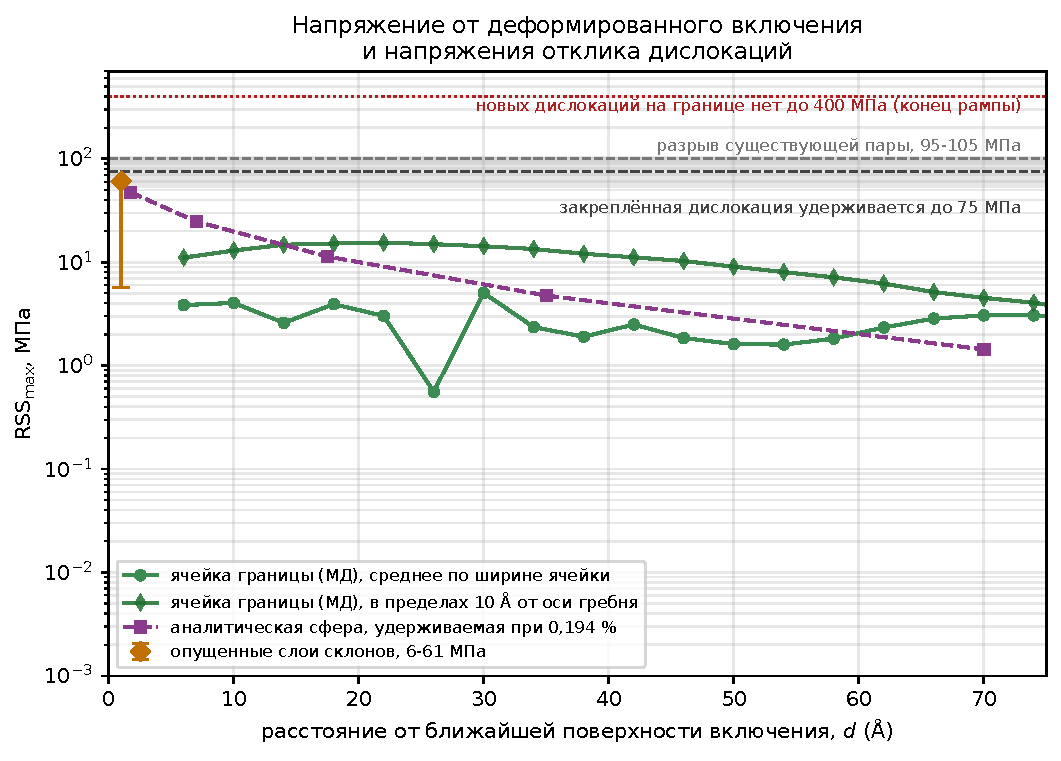
\includegraphics[width=0.9\linewidth]{fig_rss_vs_thresholds_ru}
\caption{Напряжение от деформированного включения и напряжения отклика
дислокаций: касательное напряжение, спроецированное на наиболее
благоприятную систему скольжения, $\mathrm{RSS}_{\max}$, в логарифмическом
масштабе в зависимости от расстояния $d$ до ближайшей поверхности
включения. Зелёные кружки --- ячейка границы (91\,428 атомов) с гребнем,
удерживаемым при 0{,}194\%, в среднем по ширине ячейки; зелёные ромбы --- то
же в пределах 10~\AA{} от оси гребня; для гребня $d = r - 20$~\AA{} (высота
вершины). Фиолетовые квадраты --- точное решение Эшелби [7] для сферического
включения радиуса $a = 35$~\AA{}, удерживаемого при том же удлинении в
бесконечной упругой матрице алюминия ($\mu = 26{,}5$~ГПа, $\nu = 0{,}347$,
объём-сохраняющее удлинение формулы~(1) с осью под 45$^\circ$ к $z$, тот же
максимум по двенадцати системам скольжения); для сферы $d = r - a$.
Горизонтальные линии --- конец рампы, 400~МПа, до которого новых
дислокаций на границе не образовалось (пунктир), и напряжение, при котором
приходит в движение существующая пара дислокаций (95--105~МПа), оба
из раздела~3.2; затенённая полоса $75 \pm 22$~МПа --- напряжение, выдерживаемое
закреплённой дислокацией раздела~3.3 (приложенные 75~МПа плюс-минус взаимное
напряжение пары 22~МПа с неустановленным знаком). Оранжевый ромб отмечает
диапазон, охватываемый опущенными слоями на склонах гребня; измерением поля
он не является.}
\label{fig:rss}
\end{figure}

\begin{figure}[!htbp]
\centering
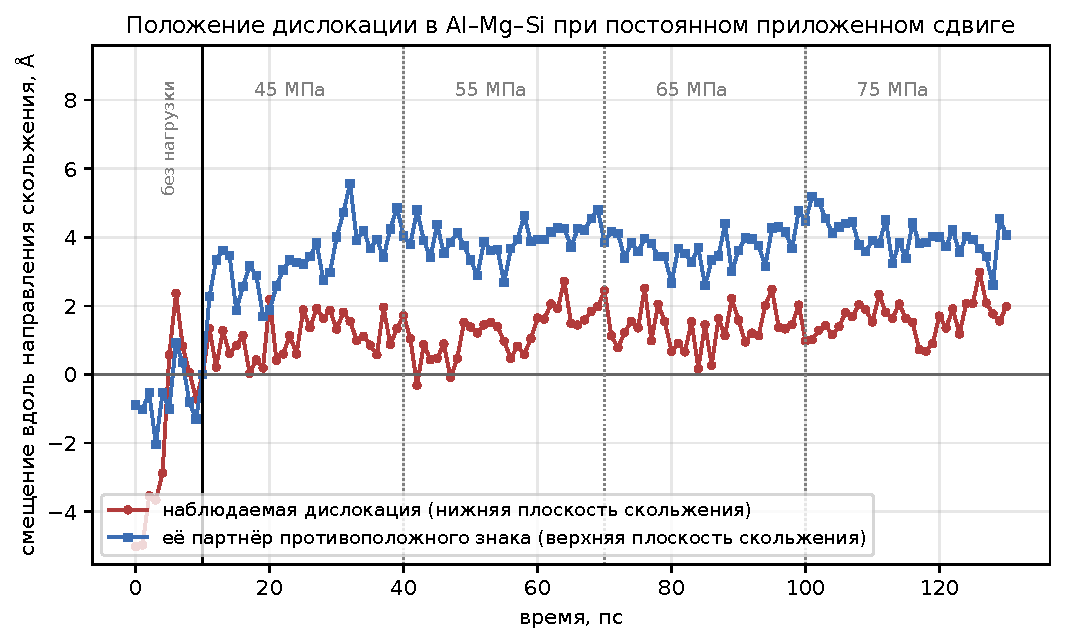
\includegraphics[width=0.9\linewidth]{fig_trajectories_ru}
\caption{Положение дислокации вдоль направления скольжения в зависимости от
времени в ячейке Al--Mg--Si при ступенчатом нагружении постоянными
приложенными сдвиговыми напряжениями (пунктир --- границы ступеней, над
каждой указано приложенное напряжение; смещение отсчитывается от положения в момент включения нагрузки,
$t = 10$~пс, после 10~пс без нагрузки). Красная кривая --- дислокация, за
движением которой велось наблюдение (нижняя в паре); синяя --- её партнёр
противоположного знака в верхней плоскости скольжения. Дислокация
колеблется около одного положения и не движется: пластического смещения
нет ни при одном из четырёх уровней напряжения. За всю историю нагружения
она смещается на 2{,}0~\AA{}, меньше одного вектора Бюргерса
$b = 2{,}86$~\AA{}, при амплитуде тепловых колебаний 0{,}6~\AA{}. Партнёр в
момент включения нагрузки выбирает 4{,}1~\AA{} ($1{,}4\,b$) и на этом
останавливается: за оставшиеся три ступени его положение меняется меньше,
чем на амплитуду его тепловых колебаний 0{,}5~\AA{}. Этот одиночный
начальный шаг не является устойчивым скольжением.
}
\label{fig:traj}
\end{figure}

\subsection{Подвижность дислокаций и закрепление примесями в сплаве}

Сопротивление, которое растворённые атомы Mg и Si оказывают движению
дислокации, измерено в ячейке сплава раздела~2.3: без включения, с
1{,}0~ат.\%~Mg и 0{,}6~ат.\%~Si, случайно замещающими алюминий, и с одной
парой краевых дислокаций противоположного знака в плоскостях скольжения,
отстоящих друг от друга на 206~\AA{}; ячейка нагружалась лестницей
постоянных приложенных сдвиговых напряжений 45, 55, 65 и 75~МПа по 30~пс
каждое. На рис.~\ref{fig:traj} показано положение дислокации, за движением
которой велось наблюдение (нижней в паре), и её партнёра в зависимости от
времени. Дислокация не скользит. За 120~пс нагружения она смещается на
2{,}0~\AA{} --- меньше одного вектора Бюргерса $b = 2{,}86$~\AA{} --- при
амплитуде тепловых колебаний 0{,}6~\AA{}; нетто-смещения внутри четырёх
ступеней, 0{,}6, 1{,}6, $-1{,}5$ и 0{,}2~\AA{} при 45, 55, 65 и 75~МПа,
сопоставимы с этими колебаниями и с напряжением не растут. Линия колеблется
около одного положения и при каждом уровне напряжения остаётся удержанной
окружающими её примесными атомами. Скорость, разумеется, можно подобрать
для каждой ступени, но при таких отношениях смещения к амплитуде колебаний
(все ниже 3) она описывала бы колебания, а не дрейф, и не приводится.
Траектория устанавливает нижнюю границу: выбранная случайная конфигурация
атомов Mg и Si удерживает дислокацию против движущего напряжения не менее
75~МПа. Это превышает 15~МПа, создаваемые удерживаемым гребнем у
своей поверхности (раздел~3.1), в 5 раз, а 41~МПа
аналитической сферы --- в 1{,}8 раза. Две дислокации пары действуют друг на
друга взаимным напряжением 22~МПа, знак которого относительно приложенного
сдвига здесь не установлен, поэтому осторожное прочтение границы ---
$75 \pm 22$~МПа с нижним краем 53~МПа, который всё ещё превышает обе
амплитуды. Граница лежит и выше оценки Лабуша
$\tau_c \approx 38$~МПа для данного содержания примесей [15,\,16] ---
среднеполевой оценки напряжения, необходимого, чтобы протащить дислокацию
сквозь случайное распределение примесных атомов, --- что согласуется с
локально более сильным, чем в среднем, расположением примесей в данной
единственной реализации.

В ячейке чистого алюминия той же геометрии дислокация движется свободно: её
положение блуждает в пределах отдельных ступеней напряжения на величину до
20~\AA{}, и за 130~пс траектории не происходит ни одного события захвата. В
рамках данной модели закрепление примесными атомами является, таким
образом, единственным представленным в этих ячейках препятствием движению
дислокаций. Количественный закон торможения дислокации в чистом алюминии
из той же геометрии получить не удалось: в отсутствие препятствий один из
членов пары достигает свободной поверхности и поглощается ею уже на первой
ступени, а блуждания оставшейся линии ограничены остаточным полем
периодической дислокационной конструкции; поэтому наблюдение закрепления в
сплаве сопоставляется с оценкой Лабуша, а не с измеренным коэффициентом
торможения. Поскольку открепления не происходит, активационный объём $V^{*}$ (объём, заметаемый сегментом дислокации при преодолении препятствия; он определяет, насколько сильно скорость скольжения откликается на напряжение) из этих расчётов извлечь нельзя. В качестве
центрального сценария используется $V^{*} = 70\,b^{3}$, полученное Soula и
соавт. для Al--Mg--Si после равноканального углового прессования [17];
поскольку состояние того материала отличается от рассматриваемого,
интервал $V^{*} = 19$--$142\,b^{3}$ [18] используется только как диапазон
чувствительности. Траектория служит лишь для оценки прочности препятствий
снизу. Кластеры Mg/Si не строились и не идентифицировались. Вторая случайная
конфигурация, рассчитанная только до ступеней 45, 55 и 65~МПа, точно так же
удерживала дислокацию на каждой достигнутой ступени; граница 75~МПа
опирается на ту единственную реализацию, которая прошла всю лестницу.

\section{От локального разрешённого сдвига к макроскопической ползучести}

Результаты раздела~3 ограничивают то, что деформированное включение
способно сделать локально. Чтобы связать их с макроскопическим наблюдением,
вопрос обращается: какое напряжение вокруг включений потребовалось бы, чтобы
повысить скорость ползучести на измеренные 25\%? Оценка, отвечающая на этот
вопрос, складывается из трёх составляющих.

Первая --- форма поля напряжений. Вне компактной частицы радиуса $a$,
сцепленной с матрицей и деформированной, упругое решение Эшелби [7] даёт
напряжение, спадающее с расстоянием $r$ от центра частицы как $(a/r)^{3}$.
Разрешённое касательное напряжение --- та часть напряжения, которая действует
толкающая дислокацию (раздел~2.4), и потому единственная
движет дислокацию, --- записывается в этой скалярной форме как
$\tau(r) = \tau_m (a/r)^{3}$, где $\tau_m$ --- его значение на поверхности
частицы. В разбавленной дисперсии с объёмной долей включений $f$ доля объёма
матрицы, в которой $|\tau|$ превышает заданный уровень $s$, равна
$F(>s) = f\,(\tau_m/s - 1)$ при $0 < s < \tau_m$ (объём самой частицы
вычтен), а распределение уровней напряжения по объёму матрицы задаётся
плотностью $p(s) = -\mathrm{d}F/\mathrm{d}s = f\,\tau_m/s^{2}$.

Вторая --- отклик скольжения дислокаций на напряжение. При комнатной
температуре дислокации преодолевают препятствия термически активированными
скачками, и локальное напряжение $\tau$ изменяет частоту скачков в
$\exp(\pm V^{*}\tau/kT)$ раз. Здесь $V^{*}$ --- активационный объём раздела~3.3 [18]. Поскольку напряжение вокруг
частицы принимает оба знака, оба направления учитываются с равным весом, и
скорость оказывается пропорциональной $\cosh(V^{*}\tau/kT)$.

Третья --- усреднение. Скорость ползучести сплава есть скорость, усреднённая
по объёму матрицы, поэтому $\cosh(V^{*}\tau/kT) - 1$ интегрируется с
плотностью $p(s)$. Относительное усиление скорости ползучести составляет
\begin{equation}
\frac{\langle\dot\varepsilon\rangle}{\dot\varepsilon_0} - 1
 = f\,x_0\!\int_{0}^{x_0}\!\frac{\cosh u - 1}{u^{2}}\,\mathrm{d}u
 = f\left[x_0\,\mathrm{Shi}(x_0) - (\cosh x_0 - 1)\right],
\qquad x_0 = \frac{V^{*}\tau_m}{kT},
\end{equation}
где $\mathrm{Shi}(x) = \int_0^x \sinh u\,\mathrm{d}u/u$ --- гиперболический
интегральный синус. Интеграл берётся до $s = 0$, то есть предполагается, что
напряжённые оболочки соседних частиц не перекрываются; обрезание его там, где
они перекрылись бы (при $u_{\min} = f x_0$, когда оболочка одной частицы
достигает соседних), понижает предсказанное усиление с 0{,}2500 до 0{,}2499 и
повышает требуемое $\tau_m$ примерно на $0{,}01\%$ при каждом $V^{*}$
табл.~\ref{tab:bridge}, так что приведённые значения сохраняются.
Соотношение~(2) --- модельная оценка чувствительности, а не извлечение
межфазного напряжения из эксперимента: оно описывает поле одной амплитудой
$\tau_m$, учитывает положительные и отрицательные напряжения с равным весом и
берёт пространственную статистику поля $(a/r)^{3}$. Существенно, что
$\tau_m$ --- амплитуда разрешённого сдвига на поверхности частицы, а не
полное межфазное напряжение, из которого в любой плоскости скольжения
действует лишь часть.

В оценку входят следующие величины. Температура --- 300~К. Содержание включений в сплаве
0{,}35~масс.\%, что отвечает объёмной доле $f = 0{,}00246$, в пределах
0{,}1--0{,}3\%, указанных в [5]; табл.~\ref{tab:bridge} рассчитана при этом
значении.
Активационный объём взят в интервале $V^{*} = 19$--$142\,b^{3}$,
охватывающем значения для алюминиевых сплавов [18], с центральным значением
$V^{*} = 70\,b^{3}$, измеренным для Al--Mg--Si [17]; из настоящих расчётов
$V^{*}$ не извлекался (раздел~3.3), поэтому интервал --- диапазон
чувствительности внутри модели, а не измеренная входная величина.

Результат сведён в табл.~\ref{tab:bridge}. Второй столбец получен приравниванием
левой части~(2) к 0{,}25 и решением относительно $\tau_m$:
8{,}4--62{,}7~МПа во всём интервале $V^{*}$, причём большие значения отвечают
меньшим активационным объёмам. Хотя при фиксированном $\tau_m$ усиление
пропорционально $f$, само $\tau_m$ находится обращением нелинейной функции и
потому не масштабируется как $1/f$: прямой пересчёт даёт 9{,}8--73{,}3~МПа
при $f = 0{,}001$ и 8{,}1--60{,}3~МПа при $f = 0{,}003$.

Далее следуют три сопоставления. Если бы 147~МПа работы [5] были
разрешённым касательным напряжением, действующим на дислокации,
соотношение~(2) предсказало бы усиление от $6{,}8\cdot10^{2}$ до
$2{,}7\cdot10^{46}$ (третий столбец), то есть по меньшей мере в
$2{,}7\cdot10^{3}$ раза больше наблюдаемых 0{,}25; 147~МПа в роли
касательного напряжения несовместимы с наблюдаемым усилением. Напряжение,
которое включение, деформированное на 0{,}194\%, создаёт в действительности,
меньше. Для сцепленной сферы, удерживаемой при этой деформации, точное
решение [7] даёт 41~МПа разрешённого сдвига внутри частицы и непосредственно у её поверхности
(раздел~3.1); при такой амплитуде соотношение~(2) даёт 0{,}045 при
$V^{*} = 19\,b^{3}$, 0{,}31 при $30\,b^{3}$ и значения, далеко превышающие
0{,}25, при больших $V^{*}$ (четвёртый столбец). Гребень ячейки границы,
удерживаемый при той же деформации, создаёт непосредственно над своей
вершиной 15~МПа разрешённого сдвига (раздел~3.1); при такой
амплитуде оценка даёт 0{,}042 при $V^{*} = 50\,b^{3}$ и
0{,}16 при $70\,b^{3}$ --- активационном объёме, измеренном для
Al--Mg--Si [17] (последний столбец). При деформации 0{,}194\%, таким
образом, напряжение вокруг включений имеет тот порядок, которого требует
оценка: наблюдаемые 0{,}25 воспроизводятся при $V^{*}$ примерно от
30 до 75$\,b^{3}$ в зависимости от того, какая из двух
амплитуд взята.

Это согласованность, а не подтверждение, по трём причинам. Оценка
экспоненциально чувствительна к произведению $V^{*}\tau_m$: удвоение $V^{*}$
при фиксированной амплитуде сдвигает предсказание на два--четыре порядка,
так что согласие фиксирует немногим больше порядка величины. Деформация
0{,}194\% --- входная величина, взятая из прежней оценки межфазного
напряжения [5], а не измеренное свойство включений; магнитострикция,
измеренная для объёмных сплавов железо--алюминий, не превышает $10^{-4}$
[11,\,12], то есть в двадцать раз меньше, и, поскольку напряжение
пропорционально деформации, включение с деформацией $10^{-4}$ создало бы на
своей поверхности не более 2~МПа, для которых соотношение~(2) даёт усиление
менее 0{,}4\% при любом $V^{*}$ из интервала. Наконец, оценка описывает
поле, существующее, пока включение деформировано; она ничего не говорит о
десятках минут, в течение которых эффект сохраняется после снятия поля
(раздел~5.3). Деформируются ли включения этого сплава на 0{,}194\% в поле
0{,}7~Тл --- вопрос, на котором упругий механизм стоит или падает, и вопрос
этот экспериментальный.

\begin{table}[!htbp]
\centering
\caption{Двухмасштабная оценка~(2) при $T = 300$~К, $f = 0{,}00246$ и
$b = 2{,}8638$~\AA{}. Второй столбец --- разрешённое касательное напряжение
$\tau_m$ на поверхности частицы, воспроизводящее измеренный прирост
ползучести 25\%. Остальные столбцы --- усиление
$\langle\dot\varepsilon\rangle/\dot\varepsilon_0 - 1$, которое
соотношение~(2) предсказывает, если бы в роли $\tau_m$ выступали 147~МПа
(прежняя оценка), 41~МПа (значение внутри аналитической сферы, удерживаемой при 0{,}194\%,
оно же --- амплитуда её дальнего поля, спадающего как обратный куб; 41{,}45
без округления) или 15~МПа (максимум на оси гребня в
ячейке границы, 15{,}45 без округления, раздел~3.1). Наблюдаемое значение --- 0{,}25.}
\label{tab:bridge}
\begin{tabular}{lcccc}
\hline
$V^{*}$ & $\tau_m$ для $+25\%$, МПа & при 147~МПа & при 41~МПа & при 15~МПа \\
\hline
$19\,b^{3}$  & 62{,}7 & $6{,}8\cdot10^{2}$  & 0{,}045 & 0{,}004 \\
$30\,b^{3}$  & 39{,}7 & $3{,}9\cdot10^{6}$  & 0{,}31 & 0{,}010 \\
$50\,b^{3}$  & 23{,}8 & $3{,}9\cdot10^{13}$ & 17 & 0{,}042 \\
$70\,b^{3}$  & 17{,}0 & $4{,}8\cdot10^{20}$ & $1{,}2\cdot10^{3}$ & 0{,}16 \\
$100\,b^{3}$ & 11{,}9 & $2{,}4\cdot10^{31}$ & $9{,}3\cdot10^{5}$ & 1{,}2 \\
$142\,b^{3}$ & 8{,}4  & $2{,}7\cdot10^{46}$ & $1{,}2\cdot10^{10}$ & 31 \\
\hline
\end{tabular}
\end{table}

\section{Обсуждение}

\subsection{Три напряжения и природа магнитной фазы}

В работе фигурируют три напряжения, и их необходимо различать. Первое ---
147~МПа работы [5]. Это оценка напряжения на поверхности включения,
полученная из индукции поля через эмпирический коэффициент; это не
измеренное напряжение, не разрешённое касательное напряжение в какой-либо
плоскости скольжения и не результат настоящих расчётов. Будь оно касательным
напряжением в плоскости скольжения, оно превышало бы 95--105~МПа,
при которых отрывается нижний партнёр дислокационной пары раздела~3.2;
поэтому нагружаемые ячейки не могут проверить эту оценку сравнением с
порогом --- они проверяют, создаёт ли деформированное включение в матрице
что-либо такого порядка.
Второе --- то, что даёт упругое включение, деформированное на 0{,}194\% и
сцепленное с матрицей. Точное решение для сцепленной сферы [7] --- без
проскальзывания по границе: атомы по обе её стороны взаимодействуют через
один и тот же потенциал, и никакого искусственного ограничения на границе
нет, --- даёт 41~МПа разрешённого сдвига внутри частицы со спадом
$(a/r)^{3}$ снаружи (рис.~\ref{fig:rss}). Третье --- поле, измеренное в
ячейке при той же удерживаемой деформации (раздел~3.1):
15~МПа разрешённого сдвига непосредственно над вершиной гребня
со спадом в пределах 80~\AA{} до $2{,}5\pm0{,}5$~МПа --- разрешающей
способности расчёта; в
среднем по ширине ячейки максимум составляет 5{,}0~МПа,
поскольку гребень занимает меньше половины этой ширины. Второе и третье
напряжения одного порядка и вместе ограничивают амплитуду, подставляемую в
соотношение~(2). Первое превышает их в 3{,}6--10 раз, потому что
$E\varepsilon$ --- напряжение стержня, удерживаемого при такой деформации, а
не включения, окружённого матрицей, которая деформируется вместе с ним.

Отдельная трудность связана с самой фазой. В исследованной партии сплава
рентгеновская дифракция определяет включения как Al$_{13}$Fe$_4$ (в
работе~[5] та же фаза записана как Fe$_4$Al$_{13}$; здесь всюду используется
обозначение Al$_{13}$Fe$_4$), а намагниченность образцов обнаруживает петлю
гистерезиса, то есть включения содержат ферромагнитную составляющую [5]; в
более ранних работах серии состав включений определён как Fe$_x$Al$_{1-x}$ с
$x = 86$--$87$~ат.\% [3,\,6]. Стехиометрический Al$_{13}$Fe$_4$, однако, не
обнаруживает магнитного упорядочения вплоть до 2~К --- ни по намагниченности,
ни по мёссбауэровским спектрам, непосредственно зондирующим магнитное
состояние атомов железа [19,\,20]: идеальное соединение не намагничивается,
и связанного с намагничиванием изменения формы у него быть не может (строго
нулевой деформации любого происхождения это, впрочем, не гарантирует).
Измеренный ферромагнетизм включений принадлежит, следовательно, не идеальной
решётке Al$_{13}$Fe$_4$, а иной их составляющей --- например, обогащённым
железом областям того типа, что отмечены в [3,\,6], --- и именно деформация
этой составляющей в поле существенна для механизма. Для включений данного
сплава эта деформация не измерена; использованные выше $10^{-4}$ ---
наибольшее значение, приведённое для массивных сплавов железо--алюминий
[11,\,12]. В расчётной ячейке включение представлено Al$_{13}$Fe$_4$ как
фазой, определённой в данной партии, с известной структурой [10];
деформация, заданная ему, принята как данное. Измерение деформации реальных
включений в поле представляется решающим экспериментальным шагом.

\subsection{О неосуществимости прямого моделирования и о том,
что МД измерить может}

Дислокация ведёт себя как линия, находящаяся под натяжением. Чтобы прогнуть
её через напряжённую область размером $L$, напряжение должно превышать
примерно $\mu b/L$, где $\mu$ --- модуль сдвига, $b$ --- вектор Бюргерса
[18]. Если бы все заявленные 147~МПа действовали как разрешённое касательное
напряжение --- предположение, наиболее благоприятное для механизма, --- этот
критерий даёт $L \approx 52$~нм (около $180\,b$), то есть ячейку примерно из
$2\cdot10^{8}$ атомов с учётом окружающей матрицы --- против примерно
$10^{5}$ атомов в ячейках настоящей работы. При 41~МПа соответствующий
размер составляет около 0{,}2~мкм, при 15~МПа --- около 0{,}5~мкм.
Прямое моделирование механизма на атомном масштабе, таким образом,
неосуществимо. Молекулярная динамика способна дать величины, которыми
оперирует описание на большем масштабе: напряжение на границе и его затухание
с расстоянием (раздел~3.1), напряжения, при которых дислокации приходят в
движение или образуются (разделы~3.2 и~3.3), и, через соотношение~(2),
проверку согласованности всей цепочки.

\subsection{Протокол магнитной памяти}

В экспериментах поле во время ползучести отсутствует. Образец выдерживается в
поле 30~мин, поле снимается, и лишь затем прикладывается нагрузка [4,\,6];
измеряется, таким образом, память о выдержке.
Всё, что делает поле, должно поэтому сохраняться десятки минут после его
снятия. Упругая деформация включения на это не способна: с исчезновением поля
включение возвращается к исходной форме, и напряжение вокруг него исчезает за
наносекунды. Настоящие расчёты содержат включение, удерживаемое при своей деформации,
пока релаксирует матрица (ячейка границы), включение, релаксировавшее из
него (свободный вариант), и нагружаемые ячейки со свободным (недеформированным) или удерживаемым
(недеформированным и деформированным) включением; ни одна из них не представляет состояния
материала после снятия поля. Десятки минут
способна сохраняться медленная перестройка атомов --- например, атомов Mg и
Si, закрепляющих дислокации (раздел~3.3), --- запущенная, пока действовало
поле. Такая перестройка в настоящей работе не установлена. Для её обоснования
потребовались бы термическая история и содержание вакансий в образцах, оценка
коэффициентов диффузии и отдельный расчёт, в котором поле включается,
выдерживается, выключается и лишь затем прикладывается нагрузка. Поэтому она
приводится здесь как одна из проверяемых гипотез, а не как результат.

\subsection{Ограничения}

Перенос полученных чисел на реальную частицу ограничивают два обстоятельства
геометрии. В ячейке включение --- гребень: выступ полуэллиптического сечения,
протяжённый вдоль $y$ через всю ячейку (раздел~2.1), а не компактная частица.
Напряжение вне такого выступа спадает с расстоянием медленнее, чем
$(a/r)^{3}$ для компактной частицы, а его дальность --- около 30~\AA{} в полную силу и 80~\AA{} в целом
(раздел~3.1) --- задаётся сечением гребня: это свойство данной ячейки, а не микронного включения, поле
которого простиралось бы соответственно дальше. Соотношение~(2) берёт
пространственную статистику из трёхмерного решения для компактной частицы, а
амплитуду --- либо из того же решения (41~МПа), либо из ячейки с гребнем
(15~МПа); эти значения различаются примерно в
2{,}7 раза, что и есть влияние геометрии, и это различие
проходит через табл.~\ref{tab:bridge} как разница двух её последних
столбцов. Двумерный упругий расчёт для одного гребня с теми же деформацией и
упругими постоянными, но в неограниченной матрице той же жёсткости, даёт
20~МПа у поверхности гребня со спадом до 5~МПа в пределах
10~\AA{}; атомистический гребень, жёстко удерживаемый на жёстком слое, даёт
меньшее значение у поверхности и более пологий профиль. Атомистическое и
континуальное описания гребня, таким образом, согласуются по величине, а
отличие от сферы --- геометрическое, а не артефакт ячейки.

Межатомный потенциал [9] выбран из-за охвата Al, Fe, Mg и Si; насколько точно
он воспроизводит границу Al/Al$_{13}$Fe$_4$, напряжение образования
дислокаций, строение ядра дислокации и закрепление атомами Mg и Si, в
настоящей работе отдельно не проверялось, поэтому абсолютные пороги следует
считать модельно зависимыми. Остаточное несоответствие двух решёток одинаково
в контрольной и деформированной ячейках и сокращается в их разности в первом
приближении; нелинейная релаксация может препятствовать точному сокращению.

Пороги раздела~3.2 --- наблюдения в одной ячейке, с одним набором начальных
скоростей атомов и одним темпом нагружения; их следует повторить с
независимыми наборами начальных скоростей и по меньшей мере при втором темпе.
Результат по закреплению опирается на два случайных расположения атомов Mg
и Si, лишь одно из которых прошло всю лестницу, и по одному набору начальных
скоростей; статистическая оценка порога закрепления
потребовала бы трёх--пяти независимых расположений и наборов скоростей. По
этой же причине закрепление приводится как наблюдение, а активационный объём
из него не извлекается. Термостат --- алгоритм, удерживающий температуру
ячейки при 300~К, --- действует на все подвижные атомы и сам может влиять на
пороги и на всплеск температуры при встрече и взаимном уничтожении двух
дислокаций; динамический участок следует
повторить либо с термостатом, выключенным после установления температуры,
либо с термостатом, действующим только на атомы у границ ячейки.

Поле представлено только механически --- деформацией включения. Механизмы, в
которых поле действует непосредственно на дислокацию или на препятствие, как
в теориях [1,\,2], остаются за рамками расчёта. Стоит отметить, что изменения
высоты барьера, которыми оперируют эти теории, 0{,}01--0{,}1~эВ, через
произведение $V^{*}\Delta\tau$ отвечают 0{,}97--9{,}7~МПа при
$V^{*} = 70\,b^{3}$ и 0{,}48--35{,}9~МПа во всём интервале $V^{*}$ ---
перекрываясь с найденными здесь напряжениями, а не совпадая с ними. Сами
напряжения вычислены из сил и положений атомов (вириальное выражение [8]) с
усреднением по слоям толщиной 4~\AA{}, параллельным границе; это приближение,
разрешающая способность которого после усреднения шести компонент тензора
по слою составляет $2{,}5 \pm 0{,}5$~МПа. Наконец, соотношение~(2) --- отдельная
модель, связывающая локальное напряжение с изменением скорости ползучести;
зависимости самих МД-порогов от темпа нагружения оно не устраняет.

\section{Заключение}

Напряжение, создаваемое деформированным включением в матрице, рассчитано в
ячейке границы Al/Al$_{13}$Fe$_4$ из 91\,428 атомов при удлинении включения
вдоль направления поля на 0{,}194\% без изменения объёма --- деформации,
отвечающей прежней оценке 147~МПа, --- при удерживаемой деформации
включения. Разрешённое касательное напряжение в матрице достигает
15~МПа непосредственно над включением и спадает до уровня
дальнего поля $2{,}5\pm0{,}5$~МПа в пределах 80~\AA{}; в среднем по ширине
ячейки максимум составляет 5{,}0~МПа. Аналитическое решение
для компактной частицы, удерживаемой при той же деформации, даёт 41~МПа
внутри неё со спадом обратно пропорционально кубу расстояния, так что для
включения микронного размера то же поле простирается на доли микрона.
Включение, которое ничто не удерживает, снимает большую часть деформации.

В нагружаемых ячейках заранее введённая пара дислокаций рядом с гребнем
разрывается при приложенном сдвиге 95--105~МПа при свободно релаксирующем включении; при удерживаемом включении деформированная и недеформированная ячейки на каждом этапе совпадают в пределах одного кадра рампы, 9~МПа; новых дислокаций на границе в недеформированной ячейке не образуется вплоть до конца рампы при 400~МПа; а случайное
расположение атомов Mg и Si удерживает дислокацию вплоть до 75~МПа.
Первые пикосекунды каждой рампы, при нулевом приложенном напряжении, отвечают на вопрос, сдвигает ли одно лишь поле деформированного гребня помещённую рядом дислокацию: один и тот же партнёр движется одинаково при деформированном и недеформированном гребне, движимый полем когерентности границы, а не деформацией гребня. Эти значения относятся к выбранным ячейкам, темпу нагружения и
потенциалу и не являются константами материала.

Двухмасштабная оценка~(2) требует разрешённого касательного напряжения
8{,}4--62{,}7~МПа на поверхности включения для повышения скорости
ползучести на 25\% при $f = 0{,}00246$ и $V^{*} = 19$--$142\,b^{3}$.
Рассчитанные амплитуды --- 41~МПа для частицы и 15~МПа для
гребня --- воспроизводят наблюдаемое усиление при $V^{*}$ от 30 до
75$\,b^{3}$, то есть в интервале, содержащем значение, измеренное для
Al--Mg--Si; 147~МПа в роли разрешённого сдвига превысили бы наблюдаемое
усиление не менее чем в $2{,}7\cdot10^{3}$ раза. Упругий механизм,
следовательно, количественно состоятелен тогда и только тогда, когда
включения деформируются в поле примерно на 0{,}2\%: магнитострикция,
измеренная для объёмных сплавов железо--алюминий, в двадцать раз меньше и
дала бы усиление менее 0{,}4\%.

Поскольку во время испытания на ползучесть поле выключено, его действие
должно сохраняться десятки минут; упругая деформация на это не способна, и в
качестве оставшейся возможности указывается медленная перестройка атомов ---
гипотеза, настоящими расчётами не проверенная. Решающими дальнейшими шагами
представляются установление ферромагнитной составляющей включений, прямое
измерение их деформации в поле и расчёт, в котором поле включается,
выдерживается, выключается и лишь затем прикладывается нагрузка.

\section*{Список литературы}

\FloatBarrier
\begin{enumerate}\setlength{\itemsep}{0pt}
\item В.\,И.~Альшиц, Е.\,В.~Даринская, М.\,В.~Колдаева, Е.\,А.~Петржик.
  Кристаллография \textbf{48}, 826 (2003).
\item M.\,I.~Molotskii. Mater. Sci. Eng. A \textbf{287}, 248 (2000).
\item A.~Skvortsov, D.~Pshonkin, E.~Kunitsyna, R.~Morgunov, E.~Beaugnon.
  J. Appl. Phys. \textbf{125}, 023903 (2019).
\item А.\,А.~Скворцов, Р.\,Б.~Моргунов, Д.\,Е.~Пшонкин и др.
  ФТТ \textbf{61}, вып.~6 (2019); Phys. Solid State \textbf{61}, 1023 (2019).
\item M.~Friha, V.\,K.~Nikolaev, A.\,A.~Skvortsov, D.\,E.~Pshonkin и др.
  J. Magn. Magn. Mater. \textbf{589}, 171532 (2024).
\item V.~Nikolaev, M.~Friha, A.\,A.~Skvortsov и др. Sci. Rep. \textbf{15},
  30585 (2025).
\item J.\,D.~Eshelby. Proc. R. Soc. Lond. A \textbf{241}, 376 (1957).
\item A.\,P.~Thompson, H.\,M.~Aktulga, R.~Berger и др. Comput. Phys.
  Commun. \textbf{271}, 108171 (2022).
\item B.~Jelinek, S.~Groh, M.\,F.~Horstemeyer и др. Phys. Rev. B
  \textbf{85}, 245102 (2012).
\item Y.~Liu, C.~Fan, Z.~Xu и др. Metals \textbf{14}, 463 (2024).
\item R.\,C.~Hall. J. Appl. Phys. \textbf{30}, 816 (1959).
\item C.~Bormio-Nunes, C.\,T.~dos Santos, M.\,B.~de Souza Dias и др.
  J. Alloys Compd. \textbf{539}, 226 (2012).
\item A.~Stukowski, V.\,V.~Bulatov, A.~Arsenlis. Modelling Simul. Mater.
  Sci. Eng. \textbf{20}, 085007 (2012).
\item A.~Stukowski. Modelling Simul. Mater. Sci. Eng. \textbf{18}, 015012
  (2010).
\item R.~Labusch. Phys. Status Solidi B \textbf{41}, 659 (1970).
\item G.\,P.\,M.~Leyson, W.\,A.~Curtin, L.\,G.~Hector, C.\,F.~Woodward.
  Nature Mater. \textbf{9}, 750 (2010).
\item A.~Soula, J.-P.~Couzini\'e, H.~Heni, J.~Bourgon, Y.~Champion,
  N.~Njah. J. Alloys Compd. \textbf{899}, 163334 (2022).
\item D.~Caillard, J.-L.~Martin. Thermally Activated Mechanisms in Crystal
  Plasticity. Pergamon, Oxford (2003).
\item K.\,E.~Avers, J.\,A.~Horn, R.~Kumar и др. Crystals \textbf{15}, 485
  (2025).
\item M.\,A.~Albedah, F.~Nejadsattari, Z.\,M.~Stadnik, J.~Przewoznik.
  J. Alloys Compd. \textbf{619}, 839 (2015).
\end{enumerate}

\section*{Доступность данных}
\begin{sloppypar}
Генераторы структур, входные файлы LAMMPS, код анализа и записи, стоящие за
каждым числом настоящей работы, находятся в открытом репозитории
\url{https://github.com/iluuua/magnetostriction-plasticity-bounds}. Каждый
рисунок и таблица строятся по JSON-записи, которую формирует один скрипт
анализа: профили напряжений рис.~\ref{fig:sigma} и атомистические кривые
рис.~\ref{fig:rss} (\path{stageG10_field_profile.py}), сохранённая доля
заданной деформации (\path{stageG12_eigenstrain_retention.py}),
аналитическая сфера (\path{stageG8_eshelby3d.py}) и двумерное решение для
гребня (\path{stageG17_ridge_continuum.py}), табл.~\ref{tab:bridge}
(\path{stageG5_two_scale_bridge.py}), траектории дислокаций
рис.~\ref{fig:traj} и граница закрепления (\path{stageG6_vstar_analysis.py},
\path{stageG7_pinning_stats.py}), пороги раздела~3.2
(\path{stageG2_depinning.py}).
Две минимизированные ячейки границы, по которым измерено поле напряжений,
приложены вместе с кодом (\path{data/stageG4_clean}); изображения
рис.~\ref{fig:cell} и \ref{fig:loading} строит
\path{stageG14_render_cells.py}.
\end{sloppypar}

\section*{Конфликт интересов}
Авторы заявляют об отсутствии конфликта интересов.

\end{document}
